\documentclass[12pt]{article}
\usepackage{latexsym, amssymb, amsmath, amsfonts, amscd, amsthm}
\usepackage {xcolor}
\usepackage{pgfplots}
\usepackage{framed}
\usepackage[margin=1in]{geometry}
\linespread{1} %Change the line spacing only if instructed to do so.

\newenvironment{problem}[2][Problem]
{
	\begin{trivlist} 
		\item[\hskip \labelsep {\bfseries #1 #2:}]
	}
{
	\end{trivlist}
	}

\newenvironment{solution}[1][Solution]
{
	\begin{trivlist} 
		\item[\hskip \labelsep {\itshape #1:}]
	}
	{
	\end{trivlist}
}

\newenvironment{collaborators}[1][Collaborator(s)]
{
	\begin{trivlist} 
		\item[\hskip \labelsep {\bfseries #1:}]
	}
	{
	\end{trivlist}
}
%%%%%%%%%%%%%%%%%%%%%%%%%%%%%%%%%%%%%%%%%%%%%%%%%%
%%%%%%%%%%%%%%%%%%%%%%%%%%%%%%%%%%%%%%%%%%%%%%%%%%
%%%%%%%%%%%%%%%%%%%%%%%%%%%%%%%%%%%%%%%%%%%%%%%%%%
%
%
%    You need only modify code below this block.
%
%
%%%%%%%%%%%%%%%%%%%%%%%%%%%%%%%%%%%%%%%%%%%%%%%%%%
%%%%%%%%%%%%%%%%%%%%%%%%%%%%%%%%%%%%%%%%%%%%%%%%%%
%%%%%%%%%%%%%%%%%%%%%%%%%%%%%%%%%%%%%%%%%%%%%%%%%%
%
\title{Assignment: Problem Set 7} %Change this to the assignment you are submitting.
\author{Name: Oleksandr Yardas} %Change this to your name.
\date{Due Date: 02/21/2018 } %Change this to the due date for the assignment you are submitting.
\begin{document}
	\maketitle
	\thispagestyle{empty}
	
	\section*{List Your Collaborators:}%Enter your collaborators names below. Do not delete extra rows.
	
	\begin{itemize}
		\begin{framed}
			\item 
			Problem 1: None
			\\\\
		\end{framed}
		\begin{framed}
			\item 
			Problem 2: None
			\\\\
		\end{framed}
		\begin{framed}
			\item 
			Problem 3: None
			\\\\
		\end{framed}
		\begin{framed}
			\item 
			Problem 4: None
			\\\\
		\end{framed}
		\begin{framed}
			\item 
			Problem 5: None
			\\\\
		\end{framed}
		\begin{framed}
			\item 
			Problem 6: Not Applicable
			\\\\
		\end{framed}
	\end{itemize}
\newpage
%
%%%%%%%%%%%%%%%
%
% Your problem statements and solutions start here.
% Use the \newpage command between problems so that
% each of your problems begins on its own page.
%
%%%%%%%%%%%%%%%
%Provide the problem statement.
\begin{problem}{1}
In each of the following cases, determine if the given function $T:\mathbb{R}^2 \to \mathbb{R}^2$ is a linear transformation. If yes, explain why. If no, provide an explicit counterexample.
\noindent
\newline
\newline
a. $T \left( \begin{pmatrix} x \\ y\end{pmatrix} \right) = \begin{pmatrix} xy \\ x+y\end{pmatrix}$
\begin{solution}
$T$ is not a linear transformation by definition because it does not preserve addition. Let $\vec{v_{1}},\vec{v_{2}} \in \mathbb{R}^2$ be arbitrary, and $\vec{v_{1}} = \begin{pmatrix} x_{1} \\ y_{1} \end{pmatrix}, \vec{v_{2}} =\begin{pmatrix} x_{2} \\ y_{2} \end{pmatrix}$. Note that:
\begin{align*}
T \left( \vec{v_{1}} + \vec{v_{2}} \right) = T \left(\begin{pmatrix} x_{1} \\ y_{1} \end{pmatrix} + \begin{pmatrix} x_{2} \\ y_{2} \end{pmatrix} \right) =&T \left(\begin{pmatrix} x_{1} + x_{2} \\ y_{1} + y_{2} \end{pmatrix} \right)\\
=& \begin{pmatrix} (x_{1} + x_{2})\cdot (y_{1} + y_{2}) \\(x_{1} + x_{2}) + (y_{1} + y_{2})\end{pmatrix}\\
=& \begin{pmatrix} x_{1}y_{1} + x_{2}y_{2} + x_{2}y_{1} + x_{1}y_{2} \\ x_{1} + y_{1} + x_{2} + y_{2} \end{pmatrix} \text{,}
\end{align*}
whereas
\begin{align*}
T \left( \vec{v_{1}} \right) +T \left( \vec{v_{2}} \right)=& T \left(\begin{pmatrix} x_{1} \\ y_{1} \end{pmatrix}\right) + T \left(\begin{pmatrix} x_{2} \\ y_{2} \end{pmatrix} \right) \\
=\begin{pmatrix} x_{1}y_{1} \\ x_{1} + y_{1} \end{pmatrix} + \begin{pmatrix} x_{2}y_{2} \\ x_{2} + y_{2} \end{pmatrix}\\
=& \begin{pmatrix} x_{1}y_{1} + x_{2}y_{2} \\ x_{1} + y_{1} + x_{2} + y_{2} \end{pmatrix}
\end{align*}
So we have that $T \left( \vec{v_{1}} + \vec{v_{2}} \right) \neq T \left( \vec{v_{1}} \right) +T \left( \vec{v_{2}} \right)$, and thus $T$ does not conserve addition. Because $\vec{v_{1}}, \vec{v_{2}}$ were arbitrary, the result follows.
\end{solution}

\noindent
\newline
\newline
b.  $T \left( \begin{pmatrix} x \\ y\end{pmatrix} \right) = \begin{pmatrix} y \sin ^2 (x^3) + y \cos ^2 (x^3)\\ y\end{pmatrix}$
\begin{solution}
$T$ is not a linear transformation because $T$ does not preserve scalar multiplication. Let $\vec{v} \in \mathbb{R}^2, r \in \mathbb{R}$ be arbitrary, and $\vec{v} = \begin{pmatrix} x \\ y \end{pmatrix}$. Note that:
\begin{align*}
T (r \cdot \vec{v}) = T (r \cdot \begin{pmatrix} x \\ y \end{pmatrix}) =& T (\begin{pmatrix} r \cdot x \\ r \cdot y \end{pmatrix})\\
=& \begin{pmatrix} (ry) \sin ^2 ((rx)^3) + (ry) \cos ^2 ((rx)^3)\\ ry\end{pmatrix}\\
=& \begin{pmatrix} ry \sin ^2 (r^3 x^3) + ry \cos ^2 (r^3 x^3)\\ ry\end{pmatrix}
\end{align*}
\[
\text{PAGE 1 OF 2 FOR PROBLEM 1}
\]
\end{solution}
%\newline
%\newline
%\newline
%\newline
%\newline
%\newline
%\[
%\text{PAGE 1 OF X FOR PROBLEM 1}
%\]
\end{problem}






\newpage
\begin{problem}{2}
Consider the linear transformation $T:\mathbb{R} ^2 \to \mathbb{R} ^2$ given by
\[
T\left(\begin{pmatrix} x \\ y\end{pmatrix} \right)=\begin{pmatrix} -y \\ -x\end{pmatrix} \text{.}
\]
Plot the values of at least 4 points and where $T$ sends them, and then use that to describe the action of $T$ geometrically.
\begin{solution}
We plot choose 4 points $(1,0),(0,1),(\frac{1}{\sqrt{2}},\frac{1}{\sqrt{2}},),(-\frac{1}{\sqrt{2}},\frac{1}{\sqrt{2}})$ and call them A1, B1, C1, and D1 respectfully. We plot where $T$ sends them below, denoted by A2, B2, C2, and D2:
\newline
\newline
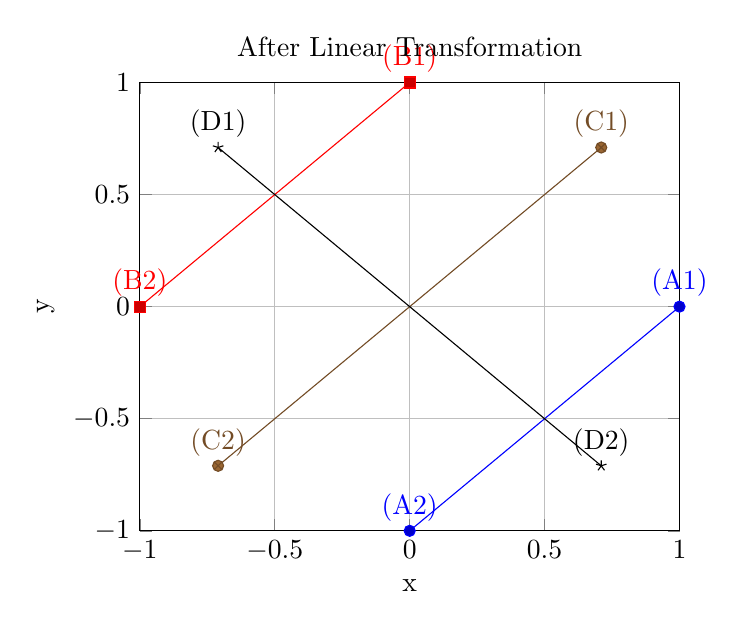
\begin{tikzpicture}
\begin{axis}[
	title = After Linear Transformation,
	xlabel = x,
	ylabel = y,
	xmin = -1, xmax = 1,
	ymin = -1, ymax = 1,
	grid=major,
	nodes near coords,enlargelimits=0
	]
\addplot+[
point meta= explicit symbolic]
	coordinates {
		(1,0) [(A1)]
		(0,-1) [(A2)]
	};
\addplot+[
point meta= explicit symbolic]
	coordinates{
		(0,1) [(B1)]
		(-1,0) [(B2)]
	};
\addplot+[
point meta= explicit symbolic]
	coordinates{
		(0.71,0.71) [(C1)]
		(-0.71,-0.71) [(C2)]
	};
\addplot+[
point meta= explicit symbolic]
	coordinates{
		(-0.71,0.71) [(D1)]
		(0.71,-0.71) [(D2)]
	};
\end{axis}
\end{tikzpicture}

It seems to be the case that $T$ is "flipping" points over the line $y=x$ about the origin. This is important because it means that points that lie on that line are also "flipped" but along the line and across the origin instead of some other point on the line.
\end{solution}
%\newline
%\newline
%\newline
%\newline
%\newline
%\newline
%\[
%\text{PAGE 1 OF X FOR PROBLEM 2}
%\]
\end{problem}






\newpage
\begin{problem}{3}
Show that the linear transformation $T:\mathbb{R} ^2 \to \mathbb{R} ^2$ given by
\[
T\left(\begin{pmatrix} x \\ y\end{pmatrix} \right)=\begin{pmatrix} x+2y \\ 3x+6y\end{pmatrix}
\]
is not injective.
\begin{solution}
We assume that $T$ is injective. Note that:
\begin{align*}
T\left(\begin{pmatrix} 1 \\ 2\end{pmatrix} \right)=&\begin{pmatrix} (1)+2(2) \\ 3(1)+6(2)\end{pmatrix}\\
=&\begin{pmatrix} 1+4 \\ 3+12\end{pmatrix}\\
=&\begin{pmatrix} 5 \\ 15\end{pmatrix} \text{,}
\end{align*}
and
\begin{align*}
T\left(\begin{pmatrix} -1 \\ 3\end{pmatrix} \right)=&\begin{pmatrix} (-1)+2(3) \\ 3(-1)+6(3)\end{pmatrix}\\
=&\begin{pmatrix} -1+6 \\ -3+18\end{pmatrix}\\
=&\begin{pmatrix} 5 \\ 15\end{pmatrix}\text{.}
\end{align*}
So we have that $T\left(\begin{pmatrix} 1 \\ 2\end{pmatrix} \right)=T\left(\begin{pmatrix} -1 \\ 3\end{pmatrix} \right)$, and note that $\begin{pmatrix} 1 \\ 2\end{pmatrix} \neq \begin{pmatrix} -1 \\ 3\end{pmatrix}$. However, we had assumed that $T$ was injective, that is that whenever $\vec{v_{1}},\vec{v_{2}} \in \mathbb{R}^2$ satisfy $T(\vec{v_{1}})=T(\vec{v_{2}})$, we have $\vec{v_{1}} =\vec{v_{2}}$. But we have just found two vectors in the domain of $T$ that do not satisfy the definition of injective, so it must be the case that $T$ is not injective.
\end{solution}
%\newline
%\newline
%\newline
%\newline
%\newline
%\newline
%\[
%\text{PAGE 1 OF X FOR PROBLEM 3}
%\]
\end{problem}






\newpage
\begin{problem}{4}
Consider the linear transformation $T:\mathbb{R} ^2 \to \mathbb{R} ^2$ given by
\[
T\left(\begin{pmatrix} x \\ y\end{pmatrix} \right)=\begin{pmatrix} 2x-y \\ -5x+3y\end{pmatrix} \text{.}
\]
Show that
\[
\begin{pmatrix} -18 \\ 47\end{pmatrix} \in \text{ range}(T)
\]
by explicitly finding $\vec{v} \in \mathbb{R}^2$ with
\[
T(\vec{v})=\begin{pmatrix} -18 \\ 47\end{pmatrix} \text{.}
\]
\begin{solution}
If $\begin{pmatrix} -18 \\ 47\end{pmatrix} \in \text{ range}(T)$, then there exists a $\vec{v} \in \mathbb{R}^2$ with $T(\vec{v}) = \begin{pmatrix} -18 \\ 47\end{pmatrix}$. So we solve for $\vec{v}$. We have:
\[
T(\vec{v}) = T\left(\begin{pmatrix} x \\ y\end{pmatrix} \right) = \begin{pmatrix} 2x-y \\ -5x+3y\end{pmatrix} = \begin{pmatrix} -18 \\ 47\end{pmatrix}
\]
So we solve for $\begin{pmatrix} x\\y \end{pmatrix}$ with $ \begin{pmatrix} 2x-y \\ -5x+3y\end{pmatrix} = \begin{pmatrix} -18 \\ 47\end{pmatrix}$. We start with the first component of the vector:
\begin{align*}
2x - y = -18\\
2x+18 =y
\end{align*}
and we substitute this $y$ into the other component,
\begin{align*}
-5x + 3 (2x +18) = 47\\
-5x + 6x + 54 =47\\
x = 47-54 =-7
\end{align*}
We have found $x=-7$. Now we solve for $y$:
\begin{align*}
y= 2*(-7) +18 = -14 +18 = 4
\end{align*}
We check our answer:
\begin{align*}
T\left(\begin{pmatrix} -7 \\ 4\end{pmatrix} \right)=&\begin{pmatrix} 2(-7)-(4) \\ -5(-7)+3(4)\end{pmatrix}\\
=& \begin{pmatrix} -14-4 \\ 35+12\end{pmatrix}\\
=&\begin{pmatrix} -18 \\ 47\end{pmatrix}
\end{align*}
We have found a $\vec{v} \in \mathbb{R}^2$, namely $\begin{pmatrix} -7 \\ 4\end{pmatrix}$, such that $T(\vec{v}) = \begin{pmatrix} -18 \\ 47\end{pmatrix}$. Therefore, $\begin{pmatrix} -18 \\ 47\end{pmatrix} \in$ range$(T)$.
\end{solution}
%\newline
%\newline
%\newline
%\newline
%\newline
%\newline
%\[
%\text{PAGE 1 OF X FOR PROBLEM 4}
%\]
\end{problem}






\newpage
\begin{problem}{5}
Suppose that $T:\mathbb{R} ^2 \to \mathbb{R} ^2$ and $S:\mathbb{R} ^2 \to \mathbb{R} ^2$ are both linear transformations. Show that $T \circ S: \mathbb{R} ^2 \to \mathbb{R} ^2$ is a linear transformation.
\begin{solution}
Let $T:\mathbb{R} ^2 \to \mathbb{R} ^2$ and $S:\mathbb{R} ^2 \to \mathbb{R} ^2$ be arbitrary linear transformations. Let $\vec{v_{1}}, \vec{v_{2}}, \vec{w} \in \mathbb{R}^2$ be arbitrary vectors.
Let $c \in \mathbb{R}$ be an arbitrary scalar.
If  $T \circ S: \mathbb{R} ^2 \to \mathbb{R} ^2$ is a linear transformation, then by the definition of a linear transformation, we have the following:
\noindent
\newline
\newline
{\it 1. } $(T \circ S)(\vec{v_{1}} + \vec{v_{2}}) = (T \circ S)(\vec{v_{1}}) + (T \circ S)(\vec{v_{2}})$
\noindent
\newline
\newline
{\it 2. } $(T \circ S)(c \cdot \vec{w}) = c \cdot (T \circ S)(\vec{w})$
\noindent
\newline
\newline
We first show that {\it 1. }is true.
\begin{align*}
(T \circ S)(\vec{v_{1}} + \vec{v_{2}}) =& T(S(\vec{v_{1}} + \vec{v_{2}})) &\text{(By definition of function composition)}\\
=& T(S(\vec{v_{1}}) + S(\vec{v_{2}})) &\text{(By definition of linear transformation)}\\
=&T(S(\vec{v_{1}})) + T(S(\vec{v_{2}})) &\text{(By definition of linear transformation)}\\
=& (T \circ S)(\vec{v_{1}}) + (T \circ S)(\vec{v_{2}}) &\text{(By definition of function composition)}
\end{align*}
Therefore, $(T \circ S)(\vec{v_{1}} + \vec{v_{2}}) = (T \circ S)(\vec{v_{1}}) + (T \circ S)(\vec{v_{2}})$, and the first condition is satisfied.
\newline
Now we show that {\it 2. }is true.
\begin{align*}
(T \circ S)(c \cdot \vec{w}) =& T(S(c \cdot \vec{w})) &\text{(By definition of function composition)}\\
=& T(c \cdot S(\vec{w})) &\text{(By definition of linear transformation)}\\
=& c \cdot T(S(\vec{w})) &\text{(By definition of linear transformation)}\\
=& c \cdot (T \circ S)(\vec{w}) &\text{(By definition of function composition)}
\end{align*}
Therefore, $(T \circ S)(c \cdot \vec{w}) = c \cdot (T \circ S)(\vec{w})$, and the second condition is satisfied. Both conditions have been satisfied, therfore the function $T \circ S: \mathbb{R}^2 \to \mathbb{R}^2$ is a linear transformation.



%\newline
%\newline
%\newline
%\newline
%\newline
%\newline
%\[
%\text{PAGE 1 OF X FOR PROBLEM 5}
%\]


\newpage

whereas
\begin{align*}
r\cdot T (\vec{v}) =& r\cdot \begin{pmatrix} y \sin ^2 (x^3) + y \cos ^2 (x^3)\\ y\end{pmatrix}\\
=& \begin{pmatrix} ry \sin ^2 (x^3) + ry \cos ^2 (x^3)\\ ry\end{pmatrix}
\end{align*}
So we have that $T (r \cdot \vec{v}) \neq r\cdot T (\vec{v})$, and thus $T$ does not conserve scalar multiplication. Because $r, \vec{v}$ were arbitrary, the result follows.
\end{solution}

\noindent
\newline
\newline
c. $T \left( \begin{pmatrix} x \\ y\end{pmatrix} \right) = \begin{pmatrix} 2x+3y \\ 1+y\end{pmatrix}$
\begin{solution}
$T$ is not a linear transformation because $T$ does not preserve scalar multiplication.  Let $\vec{v} \in \mathbb{R}^2, r \in \mathbb{R}$ be arbitrary, and $\vec{v} = \begin{pmatrix} x \\ y \end{pmatrix}$. Note that:
\begin{align*}
T (r \cdot \vec{v}) = T (r \cdot \begin{pmatrix} x \\ y \end{pmatrix}) =& T (\begin{pmatrix} r \cdot x \\ r \cdot y \end{pmatrix})\\
=& \begin{pmatrix} 2(rx)+3(ry) \\ 1+(ry)\end{pmatrix}\\
=& \begin{pmatrix} 2rx+3ry \\ 1+ry\end{pmatrix} \text{,}
\end{align*}
whereas
\begin{align*}
r \cdot T(\vec{v}) =& r \cdot \begin{pmatrix} 2x+3y \\ 1+y \end{pmatrix}\\
=& \begin{pmatrix} r(2x+3y) \\ r(1+y) \end{pmatrix}\\
=& \begin{pmatrix} 2rx+3ry \\ r+ry \end{pmatrix} \text{.}
\end{align*}
So we have that $T (r \cdot \vec{v}) \neq r\cdot T (\vec{v})$, and thus $T$ does not conserve scalar multiplication. Because $r, \vec{v}$ were arbitrary, the result follows.
\end{solution}
\noindent
\newline
\newline
\newline
\newline
\newline
\newline
\newline
\newline
\newline
\newline
\[
\text{PAGE 2 OF 2 FOR PROBLEM 1}
\]
\end{problem}




\end{document}